%----------------------------------------------------%
%              ANALISIS DE REQUISITOS                %
%----------------------------------------------------%

\chapter{Análisis de Requisitos}
\label{analisis-de-requisitos}

Este apartado contiene dos secciones mayores: el apartado \ref{analisis-de-requisitos:no-funcionales} en el que se detallan los requisitos no-funcionales y el apartado \ref{analisis-de-requisitos:funcionales} en el que se explican los requisitos funcionales recogidos de los modelos M-1 de cada UO.\\

\section{Requisitos no-funcionales}
\label{analisis-de-requisitos:no-funcionales}

La aplicación ha sido desarrollada con dos requisitos básicos:

\begin{itemize}
\item Que tenga mucha funcionalidad con el mínimo posible de \textit{clicks}.
\item Que para el alumno no suponga una distracción.
\end{itemize}

Asi pues se ha creado un diseño agradable que pretende tener mucha funcionalidad, especialmente en la vista de profesor. En la vista del alumno se ha minimizado el diseño y los elementos para que no existan distracciones importantes en clase.\\

\subsection{Requisitos de la interfaz}
\label{analisis-de-requisitos:no-funcionales:interfaz}

Para hacer más intuitiva la aplicación se han concretado unos colores e iconos específicos para cada tipo de ejercicio, de modo que sea fácil asociar una acción o estado mediante un color o un icono.

\begin{itemize}
\item Ejercicios activos: color rojo, pretendiendo indicar actividad, y un icono de un avión de papel, simbolizando un ejercicio que ha sido lanzado.
\item Ejercicios finalizados: color azul, indicando calma (ya hemos terminado), y un icono de una bandera de meta, simbolizando el fin.
\item Ejercicios preparados: color amarillo y un icono de un reloj, indicando que esto no se ha lanzado aun (viendo las aplicaciones móvil más utilizadas resulta intuitivo el significado del reloj).
\end{itemize}

Para las estadísticas se ha dejado el color verde y un icono de un gráfico de barras. El color azul se emplea para otros botones, sin usar ningún icono.\\

\section{Requisitos funcionales}
\label{analisis-de-requisitos:funcionales}

En este apartado se presentan los requisitos funcionales recogidos en interfaces de papel

Siguiendo las pautas fijadas por los requisitos no-funcionales se han realizado interfaces sencillas e intuitivas. Se le ha dado mucha importancia a la filosofía de ''en pocos \textit{clicks}'' que sigue la aplicación. Por tanto, ante todo, se han minimizado la cantidad de transiciones entre pantallas y el uso de excesivos botones para buscar mucha funcionalidad en pocos \textit{clicks}.\\

El resultado queda plasmado en estos modelos de requisitos (M-1) de cada objetivo de usuario (\textit{User Objective}). Los modelos están construidos mediante diferentes pantallas, las comunes al estudiante y al profesor son nombradas PX, donde X es el número de la pantalla, y las que son exclusivas de cada uno se denotan como \[PX_{Y}\]donde X es el número de la pantalla e Y es el usuario (puede tomar los valores S para el estudiante y T para el profesor).\\

\subsection{Requisito común: Autenticación}
\label{analisis-de-requisitos:funcionales:p1}

La autenticación es un requisito común para todos los UOs. En las figuras \ref{fig:autenticacion-alumno} y \ref{fig:autenticacion-profesor} se ve el autómata de estados correspondiente a la autenticación de un alumno y la de un profesor, respectivamente. Ambos autómatas comparten algunas pantallas, llamadas P0\textsubscript{I} y P0\textsubscript{II}, que se engloban en P0.\\

\noindent
\begin{figure}[!htbp]
\noindent
\makebox[\textwidth][c]{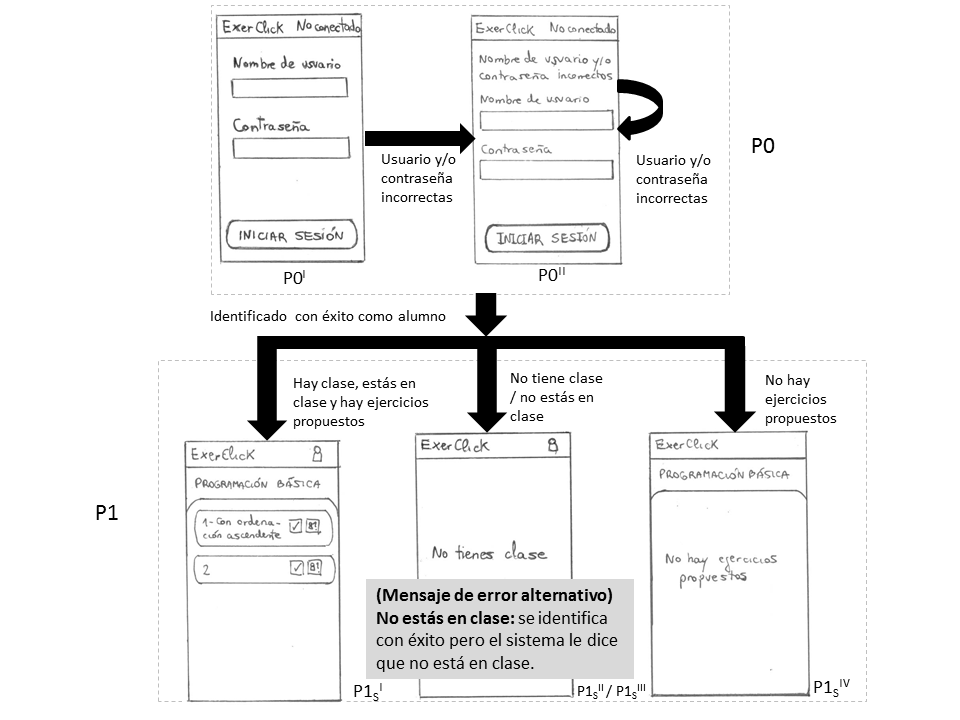
\includegraphics[width=\textwidth,keepaspectratio]{fsm2/autenticacion-s}}
\caption{Autómata de estados correspondiente a la autenticación del alumno}
\label{fig:autenticacion-alumno}
\end{figure}

\noindent
\begin{figure}[!htbp]
\noindent
\makebox[\textwidth][c]{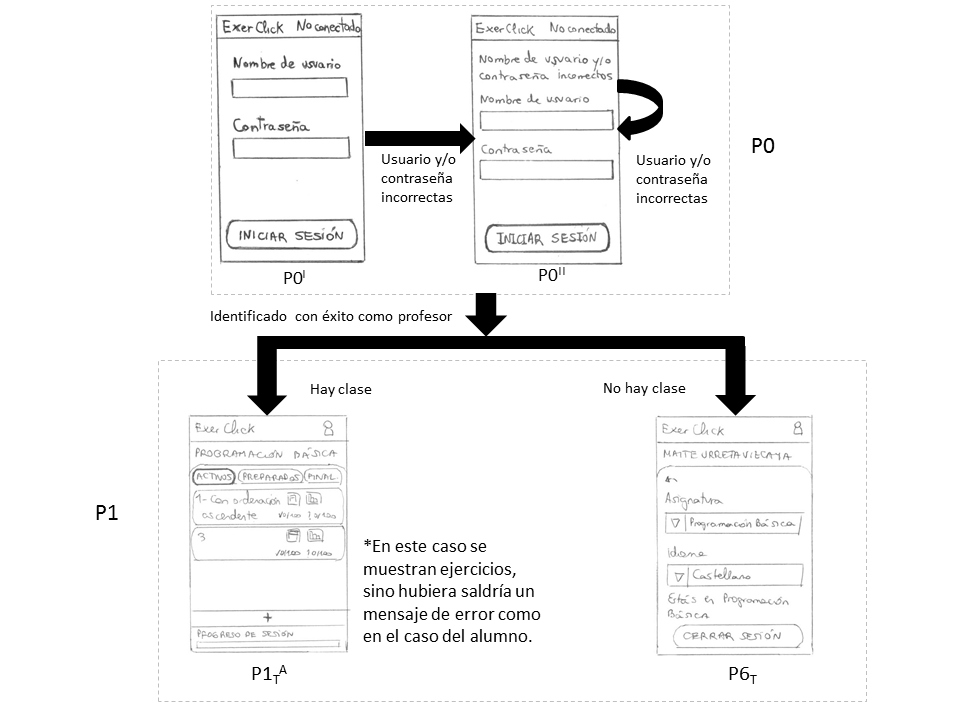
\includegraphics[width=\textwidth,keepaspectratio]{fsm2/autenticacion-t}}
\caption{Autómata de estados correspondiente a la autenticación del profesor}
\label{fig:autenticacion-profesor}
\end{figure}

En cualquier variante de P0 podemos ver dos campos para introducir nuestro nombre de usuario y contraseña y un botón para acceder. Si los datos son correctos (y tenemos clase\footnote{Se considera que hay clase desde la hora de inicio de la clase hasta la hora final y también durante 15 minutos antes de la hora de inicio}, además de estar en ella\footnote{Para reconocer que un alumno ha entrado en clase este tiene que fichar con su tarjeta de alumno.}) veremos la interfaz P1 del profesor o del estudiante (dependiendo del tipo de usuario con el que no hayamos autenticado, P1\textsubscript{S}\textsuperscript{I} para el alumno y P1\textsubscript{T}\textsuperscript{A} para el profesor). Si los datos introducidos son incorrectos iremos a P0\textsubscript{I}. También podemos ver variantes de P1 en el caso del alumno si no tenemos clase, no estamos en clase o no hay ejercicios propuestos.\\

Durante este capítulo se asumirá que el usuario se ha autenticado correctamente (como alumno o como profesor) y está en su correspondiente pantalla principal. Por tanto se obviará que todos los UOs deben pasar por P0 antes de llegar a sus pantallas iniciales.\\

\subsection{UO1-S: Responder a un ejercicio}
\label{analisis-de-requisitos:funcionales:uo1s}

El modelo M-1(1-S) requiere de la pantalla principal del alumno (P1\textsubscript{S}) Como se comentó en el apartado anterior se da por hecho que el alumno se identificó correctamente, tiene clase, está en ella y hay ejercicios propuestos. En P1\textsubscript{S} podemos responder a los ejercicios indefinidamente "sin cambiar de pantalla". No nos iremos a otra pantalla, sino que esta variará. Esta transición se puede apreciar en la figura \ref{fig:analisis-de-requisitos:funcionales:uo1s}.\\

\noindent
\begin{figure}[!htbp]
\noindent
\makebox[\textwidth][c]{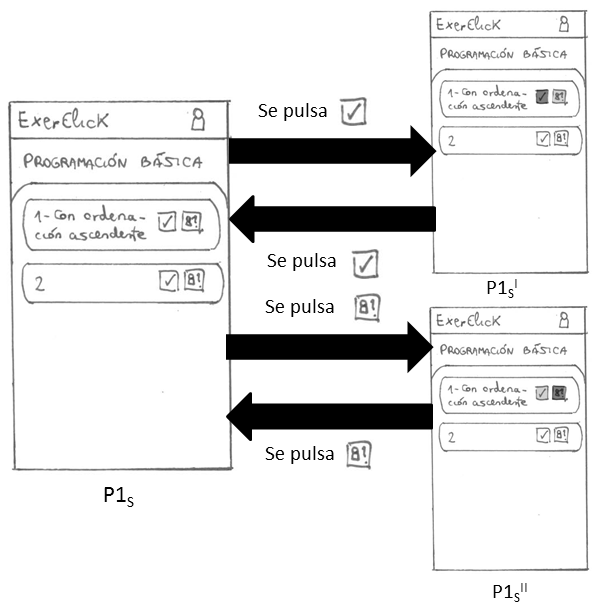
\includegraphics[width=0.7\textwidth,keepaspectratio]{fsm2/uo1s}}
\caption{Autómata de estados correspondiente al UO1-S}
\label{fig:analisis-de-requisitos:funcionales:uo1s}
\end{figure}

Nuestras opciones para responder a un ejercicio son marcar el ejercicio como finalizado (este botón será azul) o marcar una duda en el ejercicio (este será rojo). En la figura \ref{fig:analisis-de-requisitos:funcionales:uo1s} se puede ver en la parte de arriba el proceso de marcar un ejercicio como finalizado y de desmarcarlo. Análogamente para marcarlo con una duda en la parte de abajo de la misma figura.\\

\subsection{UO2-S: Ver la descripción completa de un ejercicio}
\label{analisis-de-requisitos:funcionales:uo2s}

El modelo M-1(2-S) cuenta con una pantalla P2\textsubscript{S} a la que se accede mediante P1\textsubscript{S}. En la figura \ref{fig:analisis-de-requisitos:funcionales:uo2s} se puede ver el autómata de estados correspondiente. Haciendo \textit{click} sobre el contenedor de cualquier ejercicio (sobre la ''caja'') podremos acceder a P2\textsubscript{S}. La interfaz se carga con datos sobre el ejercicio sobre el que hemos hecho \textit{click} (identificador siempre y opcionalmente cualquier otro dato que el profesor haya incluido). Si no hubiera más detalles añadidos aparecerá un mensaje avisando de ello. En P2\textsubscript{S} se aprecia un enlace ''+Más'' que estaba pensado para mostrar más detalles sobre el ejercicio. Este enlace es eliminado de aquí en adelante.\\

\noindent
\begin{figure}[!htbp]
\noindent
\makebox[\textwidth][c]{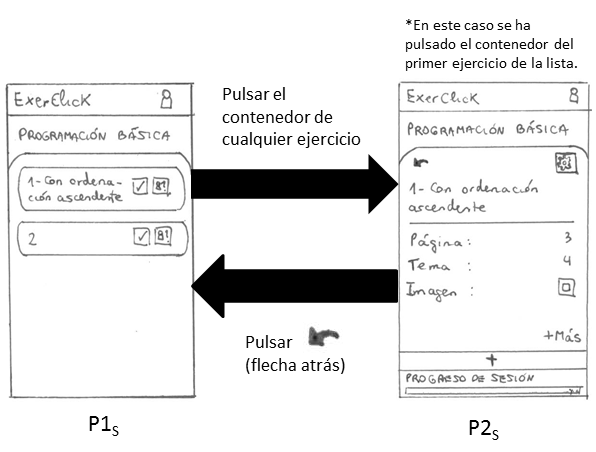
\includegraphics[width=\textwidth,keepaspectratio]{fsm2/uo2s}}
\caption{Autómata de estados correspondiente al UO2-S}
\label{fig:analisis-de-requisitos:funcionales:uo2s}
\end{figure}

\subsection{UO1-T + UO2-T: Crear-Lanzar un ejercicio simple/detallado}
\label{analisis-de-requisitos:funcionales:uo1t}

En esta sección se comentarán los UOs 1-T y 2-T, ya que el UO2-T es un modelo incremental del UO1-T, y, por tanto, están estrechamente ligados. Se comenzará hablando del UO1-T y más adelante del UO2-T.\\

\subsubsection{UO1-T: P2\textsubscript{T} (primer modelo)}

Estando en el sistema autenticados y con acceso a la asignatura, podemos crear-lanzar ejercicios pulsando en el símbolo '+', que nos da acceso a la pantalla nueva P2\textsubscript{T}, accesible desde cualquier variante de P1. En la primera versión de P2\textsubscript{T} (figura \ref{fig:analisis-de-requisitos:funcionales:uo1t:p2-viejo}) había 4 campos básicos para crear un ejercicio: un identificador, la página, el tema y una imagen. Todos los campos menos el identificador eran opcionales. Sin embargo, más tarde se pensó en reducir esto para que se viera más simple.\\

\begin{figure}[!htbp]
	\centering
	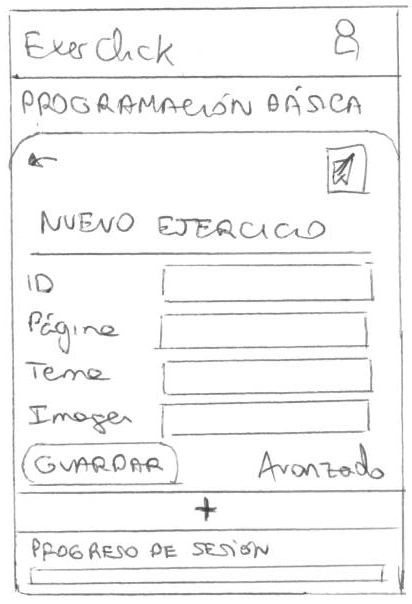
\includegraphics[height=7cm]{sheetprotos/teacher/p2-old}
	\caption{P2: Crear-Lanzar un ejercicio simple (primer modelo)}
	\label{fig:analisis-de-requisitos:funcionales:uo1t:p2-viejo}
\end{figure}

Tenemos dos botones disponibles: el de la parte superior (con un avión de papel) que lanzará directamente el ejercicio como un ejercicio activo y el de la parte inferior que guardará el ejercicio como ejercicio preparado para que podamos seguir editándolo antes de lanzarlo. Para guardar o lanzar un ejercicio es necesario que el campo del identificador no esté vacío. La flecha hacia atrás cerrará la interfaz y volveremos a P1\textsubscript{T}. Finalmente, disponemos de un enlace ''Avanzado'' que nos llevará a la interfaz P2\textsubscript{T}\textsuperscript{I}.\\

\subsubsection{UO1-T: P2\textsubscript{T} (nuevo modelo)}

En la nueva versión de la interfaz P2\textsubscript{T} (figura \ref{fig:analisis-de-requisitos:funcionales:uo1t:p2}) se utiliza la interfaz de P1, añadiendo por encima una pestaña nueva en la que podremos crear un ejercicio simple. Estos ejercicios sólo necesitan de un identificador, por tanto, en esta pequeña pestaña sólo hay un campo para añadir ese identificador. Los campos omitidos pueden ser añadidos mediante el UO2-T (en la pantalla P2\textsubscript{T}\textsuperscript{I}). Además se añade la opción de cerrar la ventana haciendo \textit{click} fuera de ésta. El enlace en el que antes ponía ''Más'' ahora por ''Avanzado'', pero en cuanto a funcionalidad sigue siendo lo mismo (muestra mas detalles para personalizar el ejercicio). Precisamente, mostrar más detalles es el objetivo del UO2-T.\\

\begin{figure}[!htbp]
	\centering
	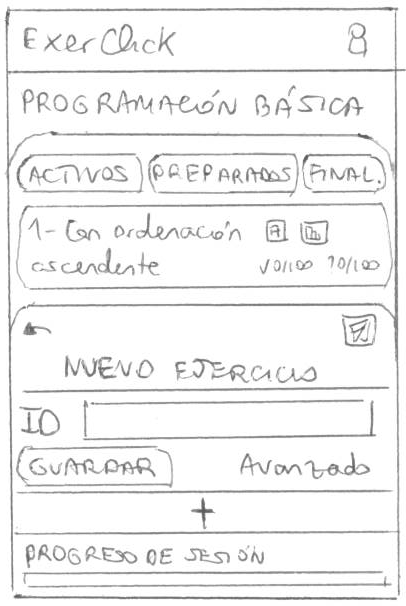
\includegraphics[height=7cm]{sheetprotos/teacher/p2}
	\caption{P2: Crear-Lanzar un ejercicio simple}
	\label{fig:analisis-de-requisitos:funcionales:uo1t:p2}
\end{figure}

\subsubsection{UO2-T}

Desde P2\textsubscript{T} es posible acceder a P2\textsubscript{T}\textsuperscript{I} pulsando sobre el enlace ''Avanzado'' (como se ha comentado previamente). Esta pantalla tiene un gran parecido con el primer modelo de P2\textsubscript{T}. Añade varios campos extra (página y tema) respecto a la nueva versión de P2\textsubscript{T}. La flecha hacia atrás cierra por completo la ventana superpuesta sobre P1\textsubscript{T}. Nuevamente el enlace ''Más'' se elimina más adelante. En la figura \ref{fig:analisis-de-requisitos:funcionales:uo1+2t:fsm} se ve el autómata de estados completo que fusiona los UOs 1-T y 2-T.\\

\noindent
\begin{figure}[!htbp]
\noindent
\makebox[\textwidth][c]{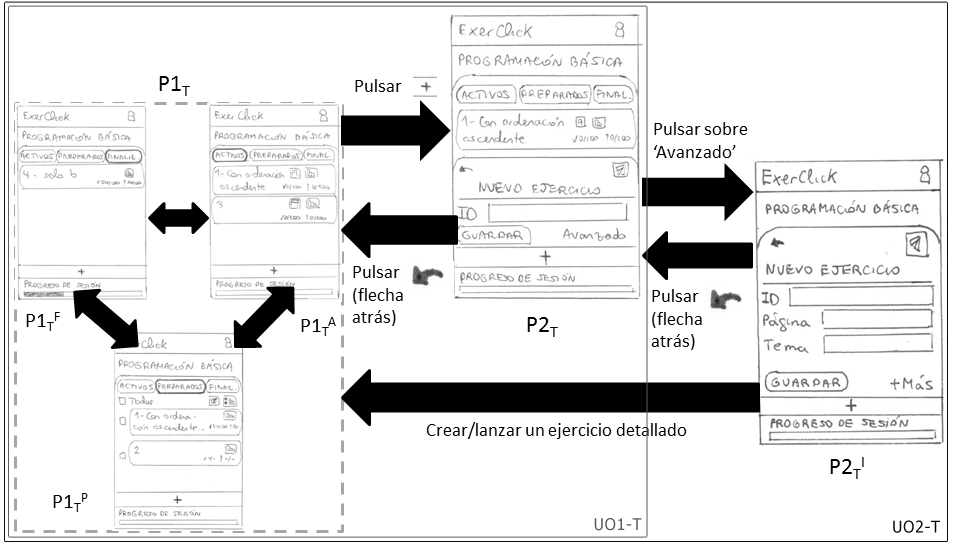
\includegraphics[width=\textwidth,keepaspectratio]{fsm2/uo1+2t}}
\caption{Autómata de estados correspondiente a los UOs 1-T y 2-T}
\label{fig:analisis-de-requisitos:funcionales:uo1+2t:fsm}
\end{figure}

\subsection{UO3-T: Cambiar el tipo de ejercicio}
\label{analisis-de-requisitos:funcionales:uo3t}

Este UO al principio tenía como finalidad cambiar un ejercicio de activo a finalizado (es decir, dar por finalizado un ejercicio propuesto en clase). Se cambió a "cambiar el tipo de un ejercicio" para dar más libertad y poder enmendar errores (ya que se daba la posibilidad de cambiar de cualquier tipo a otro). En los prototipos en papel no aparecen todos los botones, sólo la versión vieja (con el botón para finalizar ejercicios nada más).\\

Se deciden usar 3 iconos (figura \ref{fig:analisis-de-requisitos:funcionales:uo3t:iconos}) para representar cada tipo de ejercicio para que resulten intuitivos sin usar texto.\\

\begin{figure}[!htbp]
\centering
\begin{subfigure}[t]{0.3\textwidth}
	\centering
	
\includegraphics{avion-papel}
	\caption{Ejercicios activos}
	\label{fig:analisis-de-requisitos:funcionales:uo3t:iconos-1}
\end{subfigure}
%
\centering
\begin{subfigure}[t]{0.3\textwidth}
	\centering
	
\includegraphics{bandera-meta}
	\caption{Ejercicios finalizados}
	\label{fig:analisis-de-requisitos:funcionales:uo3t:iconos-2}
\end{subfigure}
%
\centering
\begin{subfigure}[t]{0.3\textwidth}
	\centering
	
\includegraphics{reloj}
	\caption{Ejercicios preparados}
	\label{fig:analisis-de-requisitos:funcionales:uo3t:iconos-3}
\end{subfigure}

\caption{Iconos utilizados para representar cada tipo de ejercicio}
\label{fig:analisis-de-requisitos:funcionales:uo3t:iconos}
\end{figure}

Desde cualquiera de las variantes de P1: P1\textsubscript{T}\textsuperscript{A} (ejercicios activos), P1\textsubscript{T}\textsuperscript{F} (ejercicios finalizados) y P1\textsubscript{T}\textsuperscript{P} (ejercicios propuestos) podemos hacer cambios. En la figura \ref{fig:analisis-de-requisitos:funcionales:uo3t:fsm} se puede ver el autómata de estados por el que se guían estos cambios.\\

\noindent
\begin{figure}[!htbp]
\noindent
\makebox[\textwidth][c]{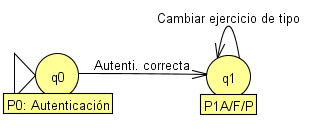
\includegraphics[width=\textwidth,keepaspectratio]{fsm2/uo3t}}
\caption{Autómata de estados correspondiente al UO3-T}
\label{fig:analisis-de-requisitos:funcionales:uo3t:fsm}
\end{figure}

Finalmente, existe una limitación a estos cambios para un caso especial. Cuando el profesor entra en la aplicación (puede hacerlo en cualquier momento, aunque no haya clase, tal y como se ve en la figura \ref{fig:autenticacion-profesor}) y quiere lanzar un ejercicio. Un requisito especial es que los ejercicios sólo pueden ser lanzados en clase. Es decir, si el profesor accede a la aplicación y no hay clase no puede crear ejercicios directamente para lanzar (UO1-T/UO2-T) ni cambiar un ejercicio al tipo activo.\\

\subsection{UO4-T: Ver estadísticas de un ejercicio}
\label{analisis-de-requisitos:funcionales:uo4t}

El profesor puede ver las estadísticas de un ejercicio, siempre y cuando sea un ejercicio activo o finalizado. Las estadísticas se muestran en tres pantallas diferentes: P2\textsubscript{T}\textsuperscript{T}, P5\textsubscript{T}\textsuperscript{A} y P5\textsubscript{T}\textsuperscript{D}.

\begin{itemize}
\item \textbf{P5\textsubscript{T}\textsuperscript{T}:} nos muestra a todos los alumnos involucrados en el ejercicios (que estén en la asignatura) en forma de lista. Muestra, por cada alumno, el estado de realización del ejercicio: acabado, con alguna duda o sin marcar nada.\\

Tanto P5\textsubscript{T}\textsuperscript{A} como P5\textsubscript{T}\textsuperscript{D} son filtros aplicados a la lista de P5\textsubscript{T}\textsuperscript{T}.
\item \textbf{P5\textsubscript{T}\textsuperscript{A}:} nos filtra sólo los alumnos que han marcado el ejercicio como acabado.
\item \textbf{P5\textsubscript{T}\textsuperscript{D}:} igual que P5A pero marcando como duda el ejercicio.
\end{itemize}

En la figura \ref{fig:analisis-de-requisitos:funcionales:uo4t:fsm} podemos ver el autómata de estados correspondiente al UO4-T.\\

\noindent
\begin{figure}[!htbp]
\noindent
\makebox[\textwidth][c]{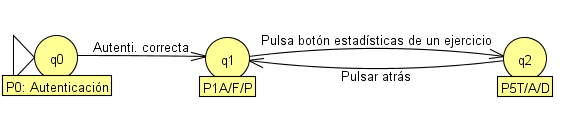
\includegraphics[width=\textwidth,keepaspectratio]{fsm2/uo4t}}
\caption{Autómata de estados correspondiente al UO4-T}
\label{fig:analisis-de-requisitos:funcionales:uo4t:fsm}
\end{figure}

Desde P1\textsubscript{T}\textsuperscript{A} o P1\textsubscript{T}\textsuperscript{F} siempre accederemos directamente a P5\textsubscript{T}\textsuperscript{T} y desde ésta podemos acceder a P5\textsubscript{T}\textsuperscript{A} y P5\textsubscript{T}\textsuperscript{D} mediante la pulsación de los botones de la parte superior. En los botones de finalizados y duda aparecen iconos, el número de acabados/dudas respecto al número de alumnos en formato n/m y el mismo dato en formato de porcentaje.\\

\subsection{UO5-T + UO6-T: Ver la descripción completa y editar un ejercicio}
\label{analisis-de-requisitos:funcionales:uo5t}

En este apartado detallaremos el análisis de requisitos de los UOs 5-T y 6-T. El UO6-T es un modelo incremental del UO5-T (al igual que los UOs 1-T y 2-T).\\

\subsubsection{UO5-T}

Es posible ver la descripción completa de un ejercicio (UO5T) desde cualquier variante de P1 (P1\textsubscript{T}\textsuperscript{A}, P1\textsubscript{T}\textsuperscript{F} o P1\textsubscript{T}\textsuperscript{P}), haciendo \textit{click} sobre el contenedor de cualquier ejercicio (sobre la ''caja'') podremos acceder a P3, tal y como se muestra en la figura \ref{fig:analisis-de-requisitos:funcionales:uo5t:fsm}. La interfaz se carga con datos sobre el ejercicio sobre el que hemos hecho \textit{click} (identificador siempre y opcionalmente cualquier otro dato que hayamos introducido como profesor). Si no hubiera más detalles añadidos aparecerá un mensaje avisando de ello.\\

Este UO es similar al UO2-S del alumno. Sin embargo, a diferencia del UO2-S (donde se mostraban también los detalles de un ejercicio) en P3 tenemos un botón con un engranaje en la parte superior, al pulsarlo nos llevará a P4 (editar el ejercicio). El enlace ''+Más'' sigue igual que en el UO2-S, sirve para mostrar más detalles. Más tarde es eliminado.\\

\noindent
\begin{figure}[!htbp]
\noindent
\makebox[\textwidth][c]{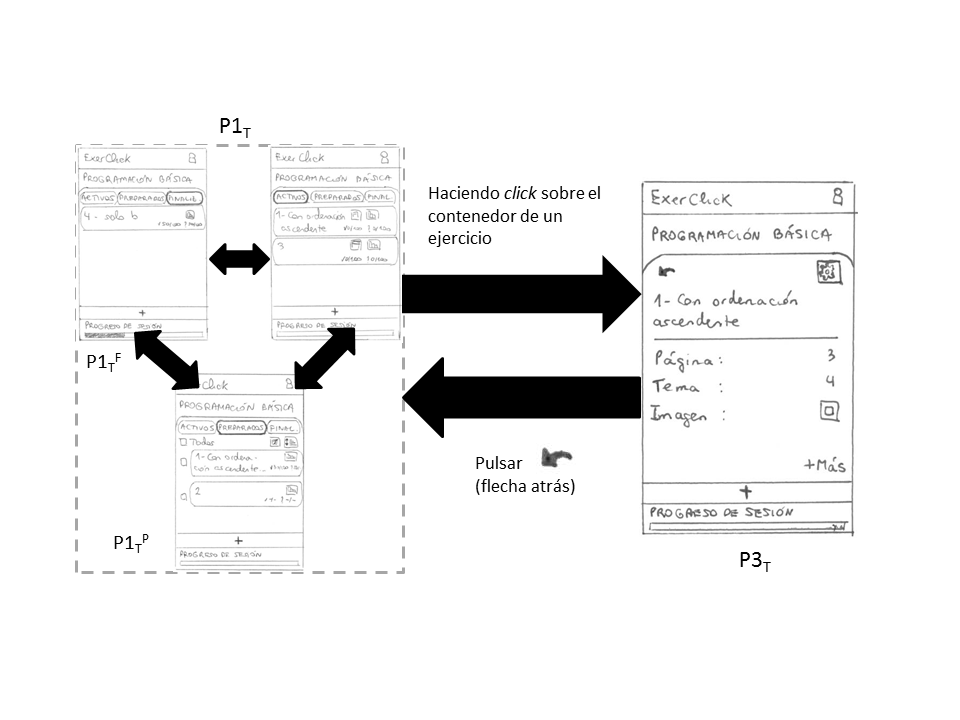
\includegraphics[width=\textwidth,keepaspectratio]{fsm2/uo5t}}
\caption{Autómata de estados correspondiente al UO5-T}
\label{fig:analisis-de-requisitos:funcionales:uo5t:fsm}
\end{figure}

\subsubsection{UO6-T}

Accederemos a P4\textsubscript{T} mediante P3\textsubscript{T} utilizando el botón con un engranaje (figura \ref{fig:analisis-de-requisitos:funcionales:uo6t:fsm}). En esta nueva pantalla podremos editar el ejercicio del que estábamos viendo los detalles en P3\textsubscript{T}.\\

En la nueva ventana tenemos el título del ejercicio y la flecha de ir atrás como en P3. En el centro de la ventana tenemos un campo por cada detalle del ejercicio, el campo se cargará con el valor previo (si tuviese). Podemos editar esos valores y pulsar el botón de ''Guardar'' para que se guarden los cambios. Si pulsamos atrás los cambios no se guardarán.\\

Más adelante el botón de atrás se elimina y se mantiene el botón de engranaje, pulsar este botón tiene el mismo efecto que la flecha para ir hacia atrás. También se cambia el título de la ventana (donde sale el título del ejercicio) por un campo con el título del ejercicio. Este campo es editable, lo cual permite editar el identificador del ejercicio (este campo no se puede dejar vacío).\\

El enlace ''Más'' muestra más detalles que editar (aunque fue eliminado más adelante).\\

\noindent
\begin{figure}[!htbp]
\noindent
\makebox[\textwidth][c]{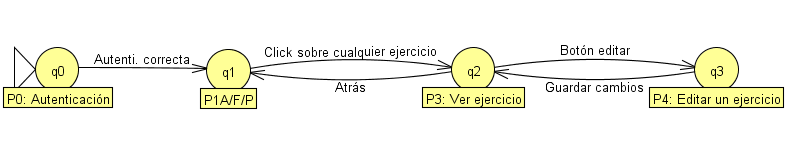
\includegraphics[width=\textwidth,keepaspectratio]{fsm2/uo6t}}
\caption{Autómata de estados correspondiente a los UOs 5-T y 6-T}
\label{fig:analisis-de-requisitos:funcionales:uo6t:fsm}
\end{figure}

\subsection{UO8-T + UO9-T + UO10-T: Cerrar sesión, Cambiar el idioma y la asignatura de la aplicación}
\label{analisis-de-requisitos:funcionales:uo8t}

La última interfaz de la aplicación es P6\textsubscript{T}. Esta interfaz es el perfil del profesor, donde se pueden realizar algunas opciones:
\begin{itemize}
\item \textbf{UO8-T:} Cerrar la sesión abierta (y volver a la pantalla inicial, P0).
\item \textbf{UO9-T:} Cambiar el idioma de la aplicación (entre Castellano, Euskera, Inglés y Francés).
\item \textbf{UO10-T:} Cambiar la asignatura activa.
\end{itemize}

Para acceder al perfil hay que hacer \textit{click} sobre el nombre de usuario o el símbolo de usuario de la parte superior derecha de la aplicación. La pantalla del perfil tiene dos desplegables (para escoger idioma y para escoger asignatura), un campo para mostrar la asignatura activa (de la que se muestran ejercicios en P1\textsubscript{T}) y un botón para cerrar sesión. Más tarde en lugar de la flecha hacia atrás que hay en la parte superior se pone un botón con el texto ''Ir a clase'' para volver a P1\textsubscript{T} (es decir, el mismo efecto que la flecha hacia atrás). En el perfil podremos realizar las acciones descritas previamente de la siguiente forma:

\begin{itemize}
\item \textbf{Cerrar sesión:} Tenemos que pulsar el botón ''Cerrar sesión'' de la parte inferior. Volveremos a P0, y desde ahí podemos autenticarnos de nuevo.
\item \textbf{Cambiar de idioma:} En el perfil del profesor aparecerá una opción ''Idioma'' con un desplegable. Al escoger cualquier opción de este la aplicación cambiará automáticamente de idioma (no hay transición de pantallas).
\item \textbf{Cambiar de asignatura:} Existe otra opción con desplegable llamada ''Asignatura'', donde podemos escoger entre cualquier asignatura del profesor. Al escoger una nueva asignatura no se apreciarán más cambios que el texto que aparece sobre el botón de cerrar sesión (donde aparece la asignatura que está seleccionada), sin embargo la ''asignatura activa'' ha cambiado. Es decir, si volvemos de nuevo a los ejercicios (P1\textsubscript{T}) veremos que estamos en la nueva asignatura seleccionada, y, por tanto, aparecerán los ejercicios de esa asignatura.\\
\end{itemize}

Todo se resume en el autómata de estados de la figura \ref{fig:analisis-de-requisitos:funcionales:uo8-9-10t:fsm}, donde aparecen las transiciones de los 3 UOs.\\

\noindent
\begin{figure}[!htbp]
\noindent
\makebox[\textwidth][c]{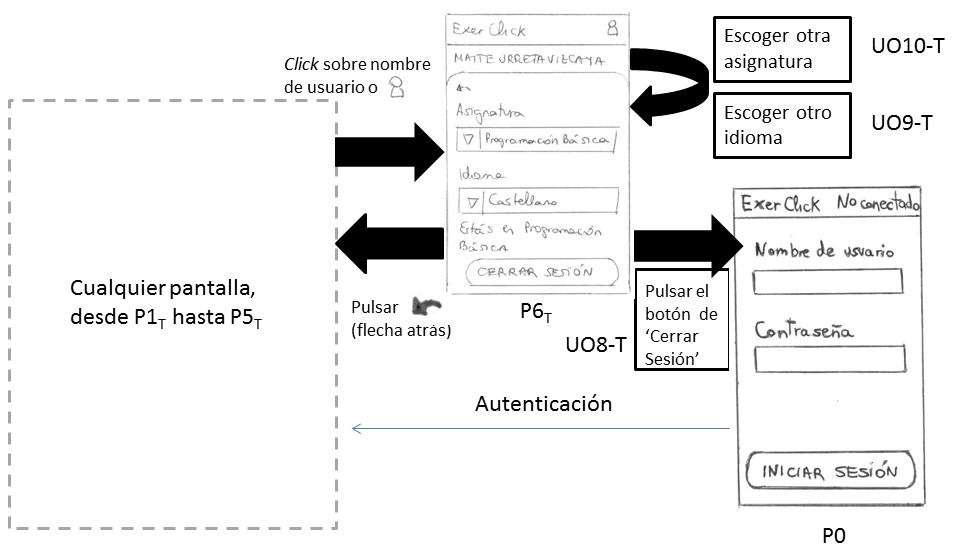
\includegraphics[width=\textwidth,keepaspectratio]{fsm2/uo8-9-10t}}
\caption{Autómata de estados correspondiente a los UOs 8-T, 9-T y 10-T}
\label{fig:analisis-de-requisitos:funcionales:uo8-9-10t:fsm}
\end{figure}

%\subsection{UO1: Lanzar ejercicios}
%\label{analisis-de-requisitos:funcionales:uo1}

%\noindent
%\begin{figure}[!htbp]
%\noindent
%\makebox[\textwidth][c]{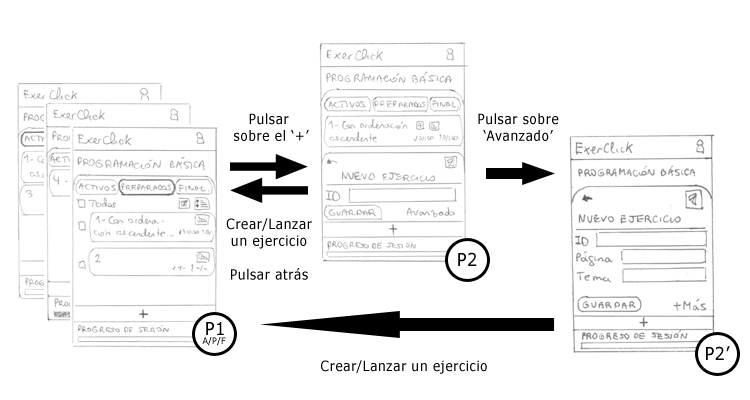
\includegraphics[width=\textwidth,keepaspectratio]{fsm2/uo1}}
%\caption{Autómata de estados correspondiente al UO1}
%\label{fig:analisis-de-requisitos:funcionales:uo1:fsm}
%\end{figure}

%Este modelo es una combinación de los UO1-T (Crear-lanzar un ejercicio simple) y UO2-T (Crear-lanzar un ejercicio %avanzado), permite crear un ejercicio simple o uno avanzado (dependiendo de las necesidades del profesor).\\

%\subsection{UO2: Lanzar ejercicios y visualizar resultados}
%\label{analisis-de-requisitos:funcionales:uo2}

%\noindent
%\begin{figure}[!htbp]
%\noindent
%\makebox[\textwidth][c]{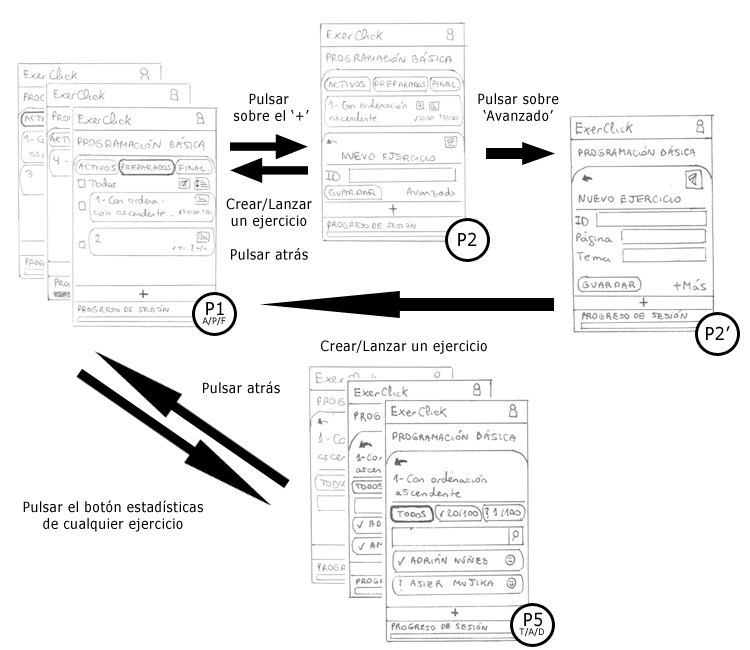
\includegraphics[width=\textwidth,keepaspectratio]{fsm2/uo2}}
%\caption{Autómata de estados correspondiente al UO2}
%\label{fig:analisis-de-requisitos:funcionales:uo2:fsm}
%\end{figure}

%Combinando el UO1 anterior con el UO4-T (ver estadísticas de un ejercicio) obtenemos el UO2 de la figura %\ref{fig:analisis-de-requisitos:funcionales:uo2:fsm}.\\